\chapter{実験1における$sin$波の再現例}

\begin{figure}[ht]
  \begin{center}
    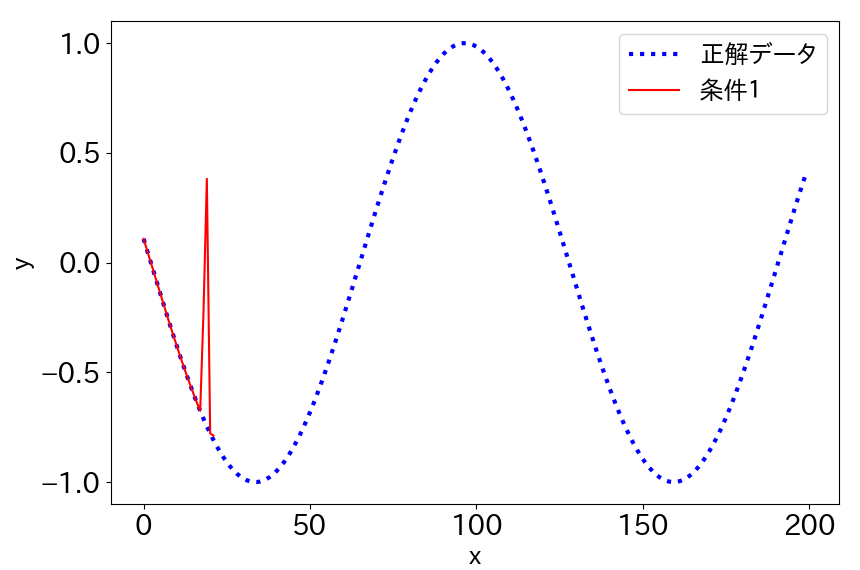
\includegraphics[width=12cm]{./fig/append1}
    \caption{条件1における再現例1}
    \label{fig:append1}
  \end{center}
\end{figure}

\begin{figure}[htp]
  \begin{center}
    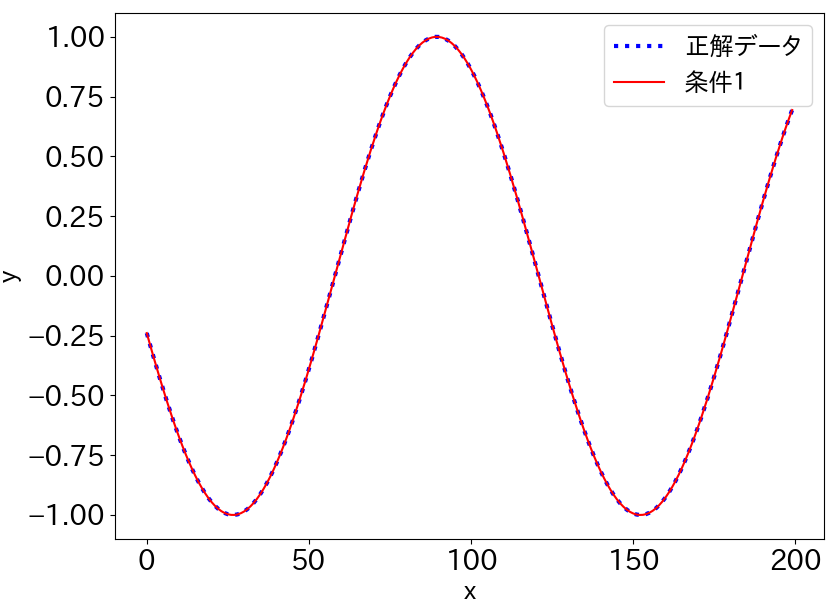
\includegraphics[width=12cm]{./fig/append2}
    \caption{条件1における再現例2}
    \label{fig:append2}
  \end{center}
\end{figure}

\begin{figure}[hp]
  \begin{center}
    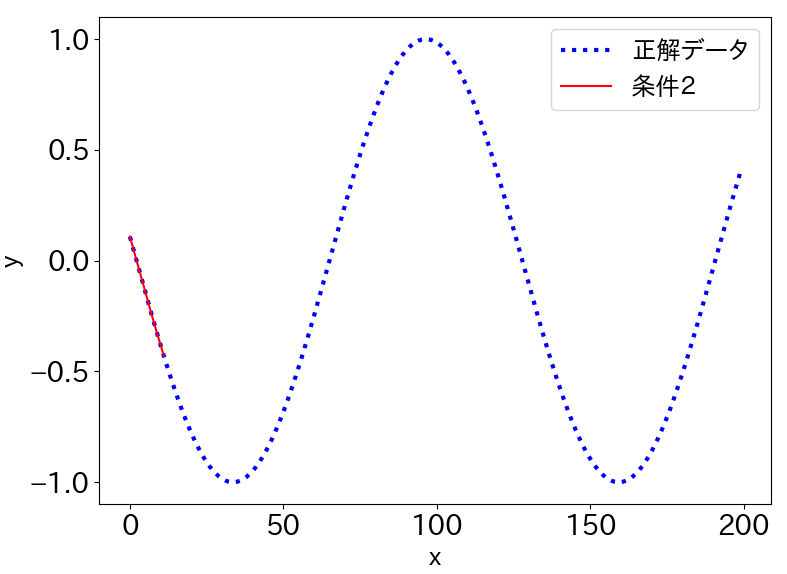
\includegraphics[width=12cm]{./fig/append3}
    \caption{条件2における再現例1}
    \label{fig:append3}
  \end{center}
\end{figure}

\begin{figure}[htp]
  \begin{center}
    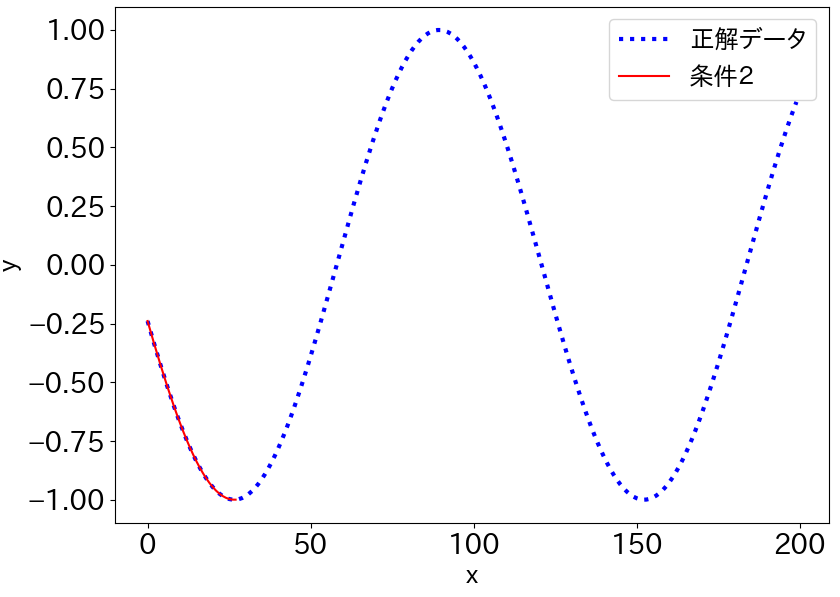
\includegraphics[width=12cm]{./fig/append4}
    \caption{条件2における再現例2}
    \label{fig:append4}
  \end{center}
\end{figure}

\begin{figure}[hp]
  \begin{center}
    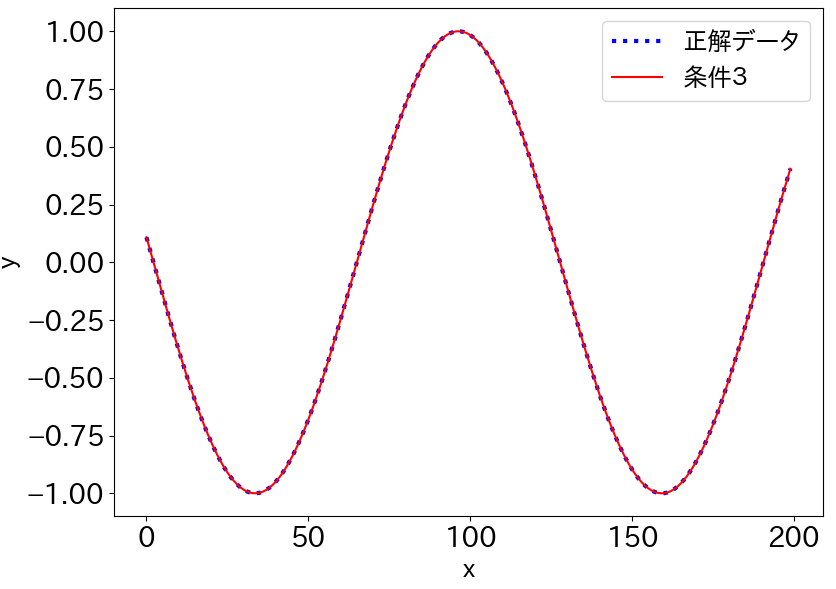
\includegraphics[width=12cm]{./fig/append5}
    \caption{条件3における再現例1}
    \label{fig:append5}
  \end{center}
\end{figure}

\begin{figure}[htp]
  \begin{center}
    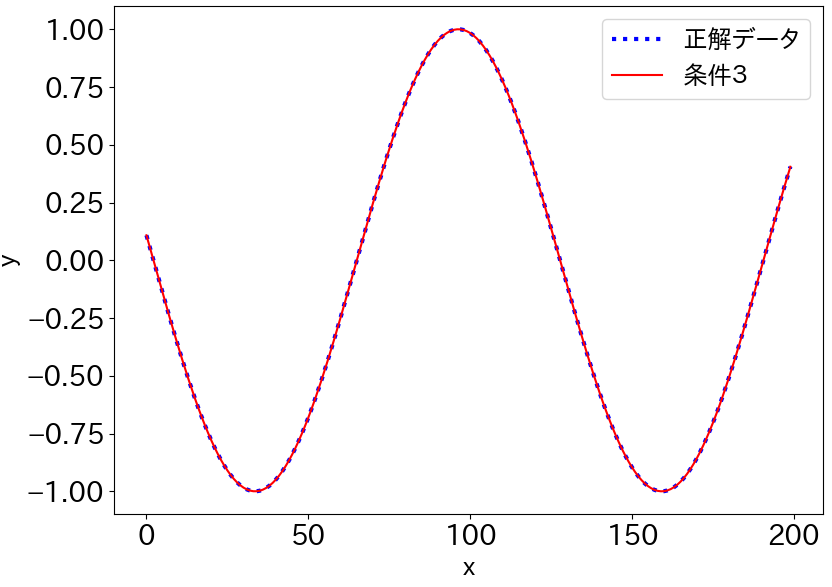
\includegraphics[width=12cm]{./fig/append6}
    \caption{条件3における再現例2}
    \label{fig:append6}
  \end{center}
\end{figure}

\begin{figure}[hp]
  \begin{center}
    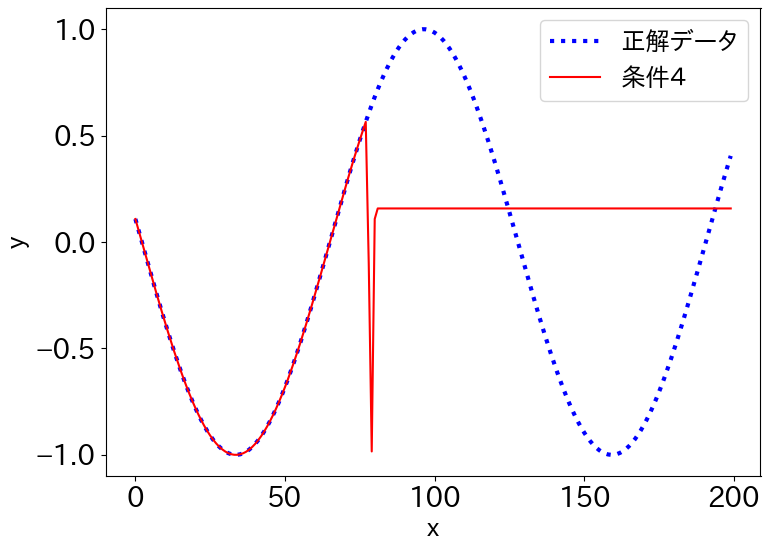
\includegraphics[width=12cm]{./fig/append7}
    \caption{条件4における再現例1}
    \label{fig:append7}
  \end{center}
\end{figure}

\begin{figure}[htp]
  \begin{center}
    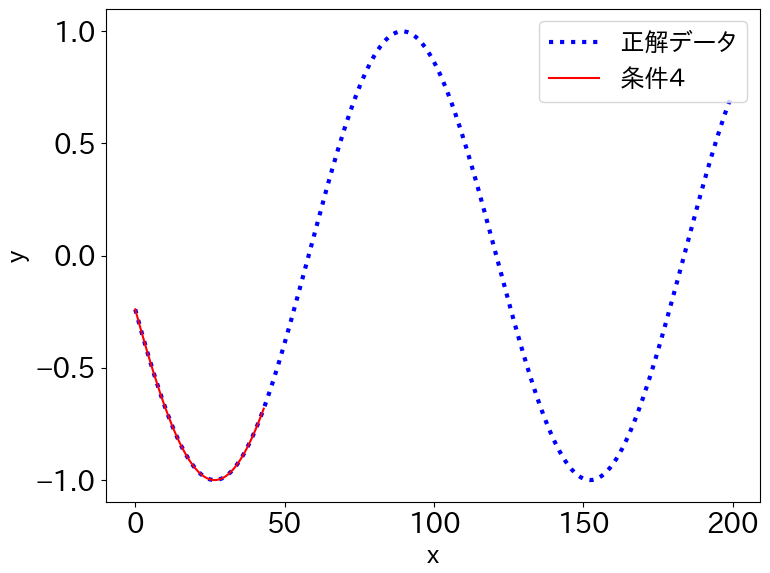
\includegraphics[width=12cm]{./fig/append8}
    \caption{条件4における再現例2}
    \label{fig:append8}
  \end{center}
\end{figure}

\begin{figure}[hp]
  \begin{center}
    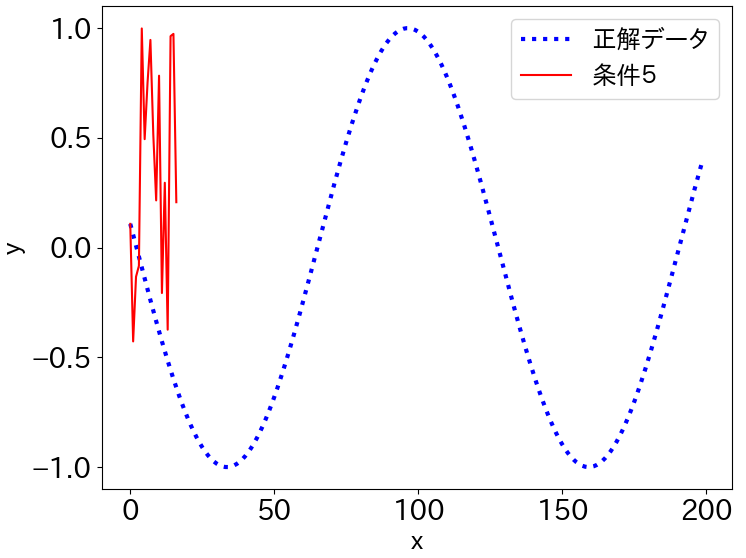
\includegraphics[width=12cm]{./fig/append9}
    \caption{条件5における再現例1}
    \label{fig:append9}
  \end{center}
\end{figure}

\begin{figure}[ht]
  \begin{center}
    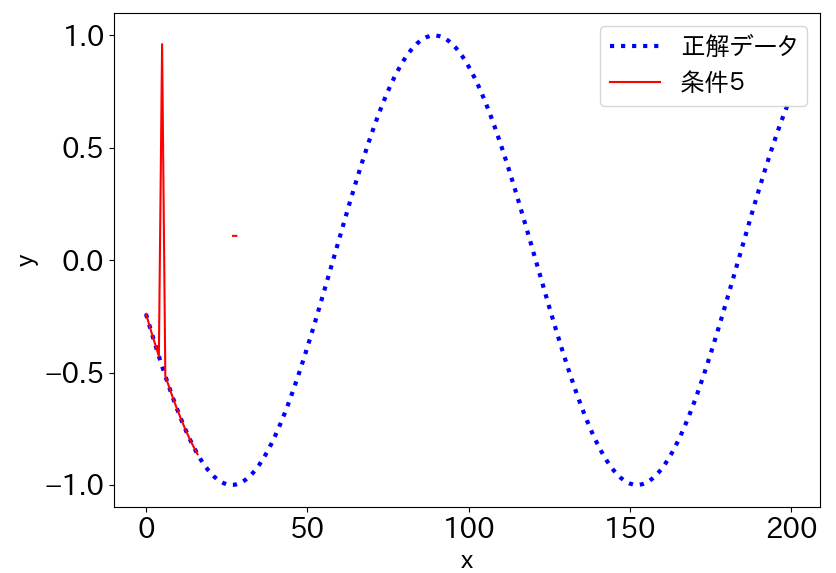
\includegraphics[width=12cm]{./fig/append10}
    \caption{条件5における再現例2}
    \label{fig:append10}
  \end{center}
\end{figure}

\newpage
図A.1\~A.10を見ると条件3以外において予測が途中で停止していることが見受けられる。
これは予測状態に遷移するセルの量が徐々に減少していき、最終的になくなっているためである。
また正解データ以外の値を取るときに大きく離れた値をとっている傾向もある。
これは入力の値をHTMのカラムの組み合わせの表現に割り当てたときに、入力の値上では近い値同士でもHTMのカラムの組み合わせの表現上では大きく離れた値に位置しているためだと考えられる。
この改善案として単層ニューラルネットワークなどを用いて入力の値の値同士の近さとHTMのカラムの組み合わせの表現における値の値同士の近さが同じになるような学習を加えるというものが考えられる。
これを今後の課題としたい。

HTMにおいてカラムの数は表現力に直接影響するためカラム数を減らした実験5では予測が正解データから大きく離れてしまっている。
また逆にカラム数が大きくなるほど多くの複雑なデータを扱えるようになるため、今後は実装上の努力によってより大きなカラム数で実行していきたい。
